\documentclass[../notes.tex]{subfiles}

\pagestyle{main}
\renewcommand{\chaptermark}[1]{\markboth{\chaptername\ \thechapter\ (#1)}{}}
\setcounter{chapter}{6}

\begin{document}




\chapter{Radicals}
\setcounter{section}{37}
\section{Radicals - 1}
\begin{itemize}
    \item \marginnote{12/9:}Grade cutoffs on Exam 4.
    \begin{itemize}
        \item A: 75-100.
        \item B: 60-74.
        \item C: 50-59.
        \item $<\text{C}$: $<50$.
        \item Speak with your TF first (then Prof. Buchwald) if you didn't do as well as you would like.
    \end{itemize}
    \item Announcements.
    \begin{itemize}
        \item The final exam is the last possible final exam: Friday, 12/20, 1:30 PM, 50-340.
        \item Syllabus update: Instead of rushing through two topics, Prof. Buchwald decided to focus more intently on one topic (radicals) for the last two lectures.
    \end{itemize}
    \item Lecture outline.
    \begin{enumerate}[label={\Alph*.}]
        \item Introduction.
        \begin{itemize}
            \item Definition.
            \item Structure.
            \item Stability and stabilization.
            \item Generation.
        \end{itemize}
        \item Reactions of radicals.
        \begin{enumerate}[label={\arabic*)}]
            \item Termination steps.
            \begin{enumerate}[label={\alph*)}]
                \item Radical-radical coupling.
                \item Disproportionation.
            \end{enumerate}
            \item Propagation steps.
            \begin{enumerate}[label={\alph*)}]
                \item Abstraction.
                \item Addition to double and triple bonds.
                \item Fragmentation.
                \item Rearrangement.
            \end{enumerate}
            \item Radical chain reactions.
        \end{enumerate}
    \end{enumerate}
    \pagebreak
    \item We'll begin with Topic A: Introduction.
    \item \textbf{Radical}: A neutral, carbon-centered (for the sake of this class) species that can be characterized by electron spin resonance (ESR).
    \begin{figure}[h!]
        \centering
        \footnotesize
        \chemfig{R-[:30]\charge{90=\.}{}(<[:-50]R')<:[:-10]R''}
        \caption{A radical.}
        \label{fig:rad}
    \end{figure}
    \begin{itemize}
        \item ESR is also beyond the scope of this class; it is analogous to NMR if you are curious.
        \item Reading: Chapter 37 of \textcite{bib:Clayden}.
    \end{itemize}
    \item Structure of radicals.
    \begin{figure}[h!]
        \centering
        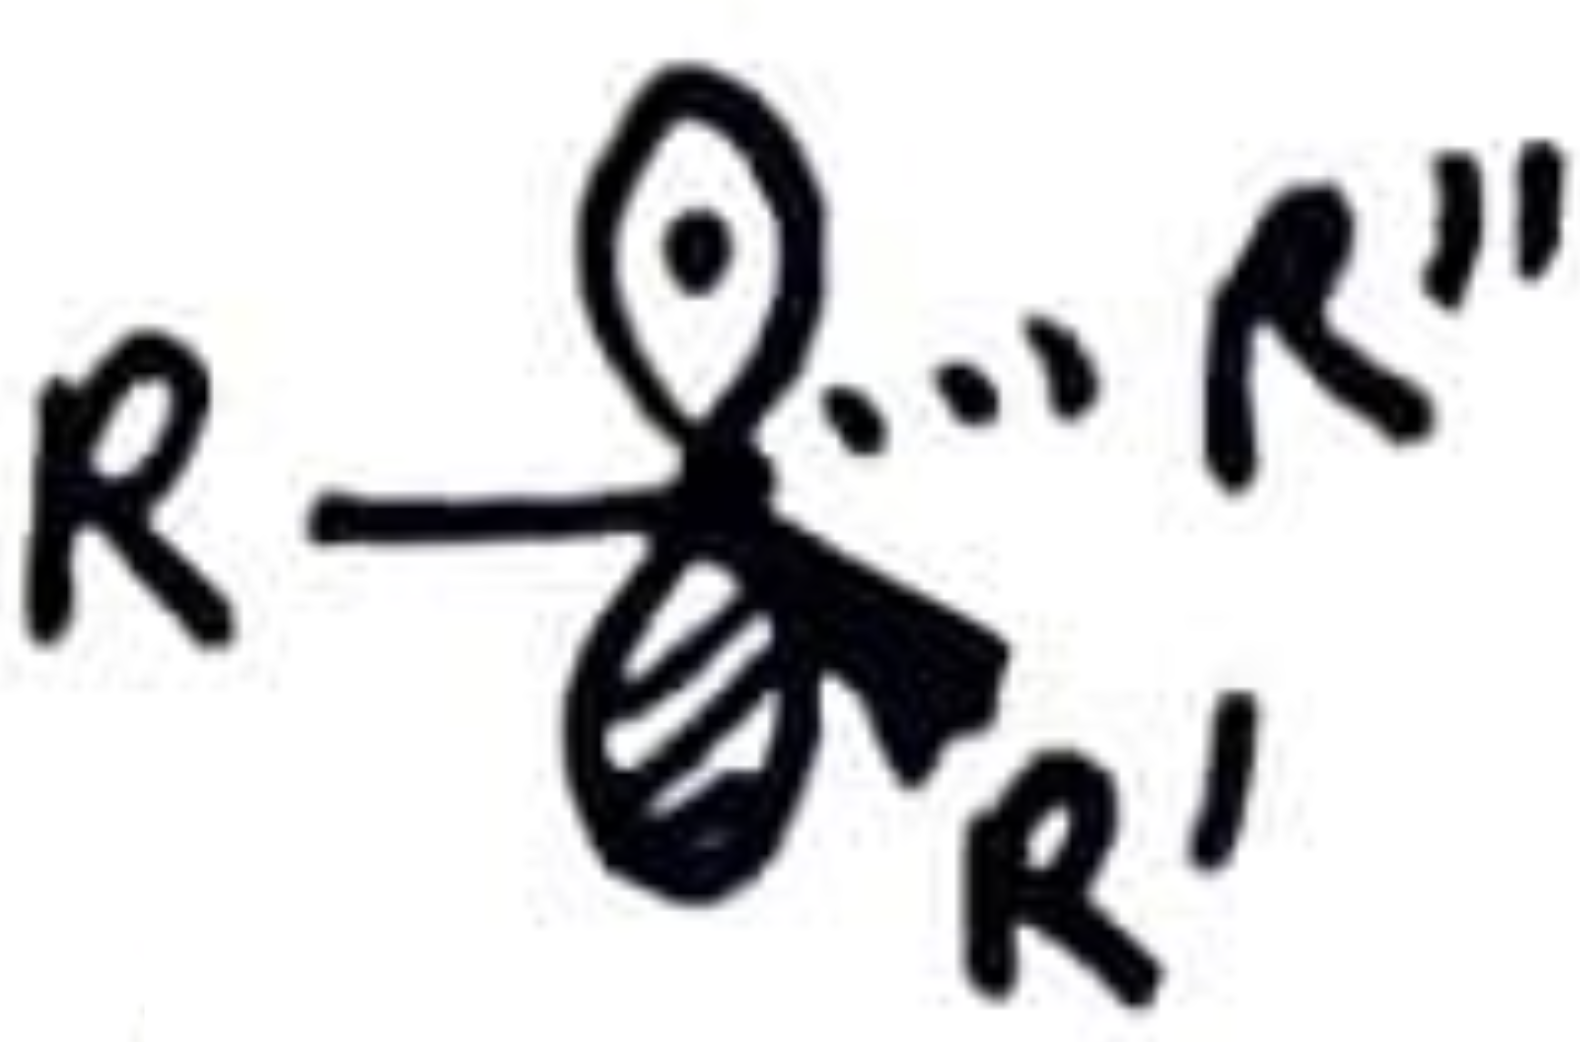
\includegraphics[width=0.1\linewidth]{radStructure.png}
        \caption{Radical structure.}
        \label{fig:radStructure}
    \end{figure}
    \begin{itemize}
        \item The carbon center is $sp^2$-hybridized.
        \begin{itemize}
            \item It is approximately planar (aka a "shallow pyramid," but we don't have to worry about that).
            \item It is subject to stereochemical "umbrella-ing": When $sp^3$-hybridized, radicals rapidly invert, like an umbrella in a windstorm.
        \end{itemize}
        \item Thus, for our purposes, there are no enantiomerically enriched radicals.
        \begin{itemize}
            \item Aside: It is a trend in modern research to take things that are unstable and stabilize them, e.g., via binding to a transition metal.
            \item People are designing molecules that can selectively bond to one face of a radical over another.
            \item All of this is way beyond the scope of this class.
        \end{itemize}
    \end{itemize}
    \item Stability of radicals.
    \begin{itemize}
        \item Radicals are electron-deficient, so methods of donating electron density into the partially filled orbital are typically the most useful at stabilizing them.
    \end{itemize}
    \item Hyperconjugative stabilization.
    \begin{equation*}
        3^\circ > 2^\circ > 1^\circ > \ce{Me}
    \end{equation*}
    \begin{itemize}
        \item It's about a \kcal{3} difference between $3^\circ$ and $2^\circ$, and between $2^\circ$ and $1^\circ$.
        \item However, it's about a \kcal{6} difference between $1^\circ$ and methyl.
        \item These differences roughly correlate with the number of hyperconjugative, no-bond resonance structures.
        \begin{itemize}
            \item 9 such structures for $3^\circ$, 6 for $2^\circ$, 3 for $1^\circ$, and 0 for methyl.
            \item Analogously to Figure \ref{fig:hyperconjugationCCa}, each methyl group adjacent to the radical adds three \ce{C-H} bonds that can donate into the partially filled radical $p$-orbital.
        \end{itemize}
    \end{itemize}
    \item Heteroatom destabilization.
    \begin{equation*}
        \ce{R3C*} > \ce{R2N*} > \ce{RO*}
    \end{equation*}
    \begin{itemize}
        \item Note that since radicals are electron deficient, carbon-centered radicals are also more stable than radicals centered on more electronegative elements.
    \end{itemize}
    \pagebreak
    \item Resonance stabilization.
    \begin{figure}[h!]
        \centering
        \begin{subfigure}[b]{0.32\linewidth}
            \centering
            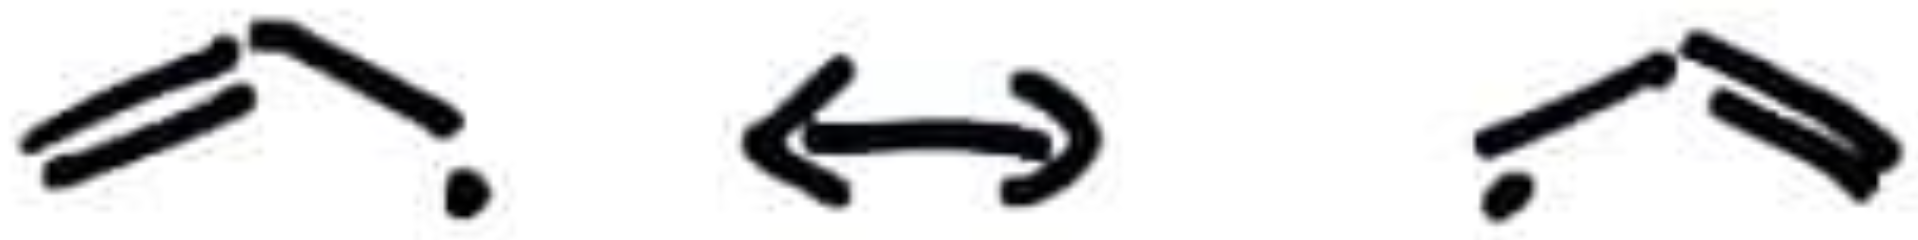
\includegraphics[width=0.65\linewidth]{radResa.png}
            \caption{Allyl radical.}
            \label{fig:radResa}
        \end{subfigure}
        \begin{subfigure}[b]{0.32\linewidth}
            \centering
            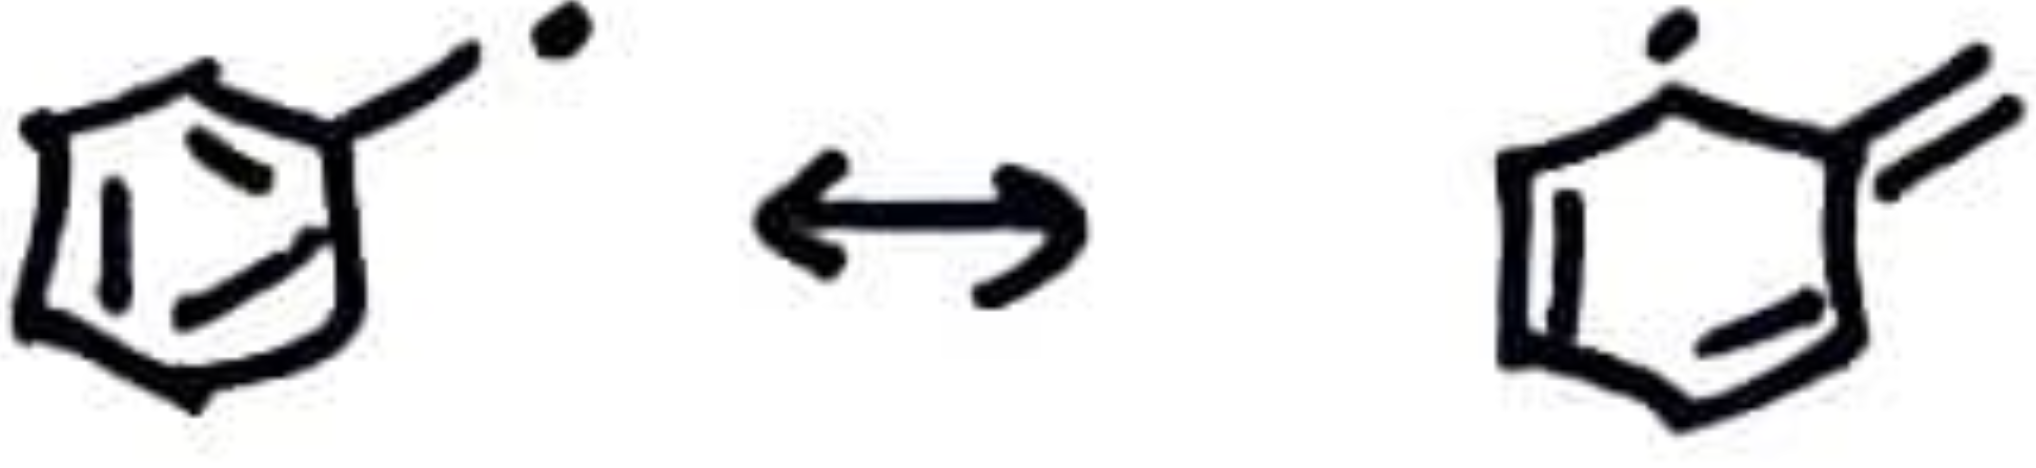
\includegraphics[width=0.7\linewidth]{radResb.png}
            \caption{Benzyl radical.}
            \label{fig:radResb}
        \end{subfigure}\\[2em]
        \begin{subfigure}[b]{0.32\linewidth}
            \centering
            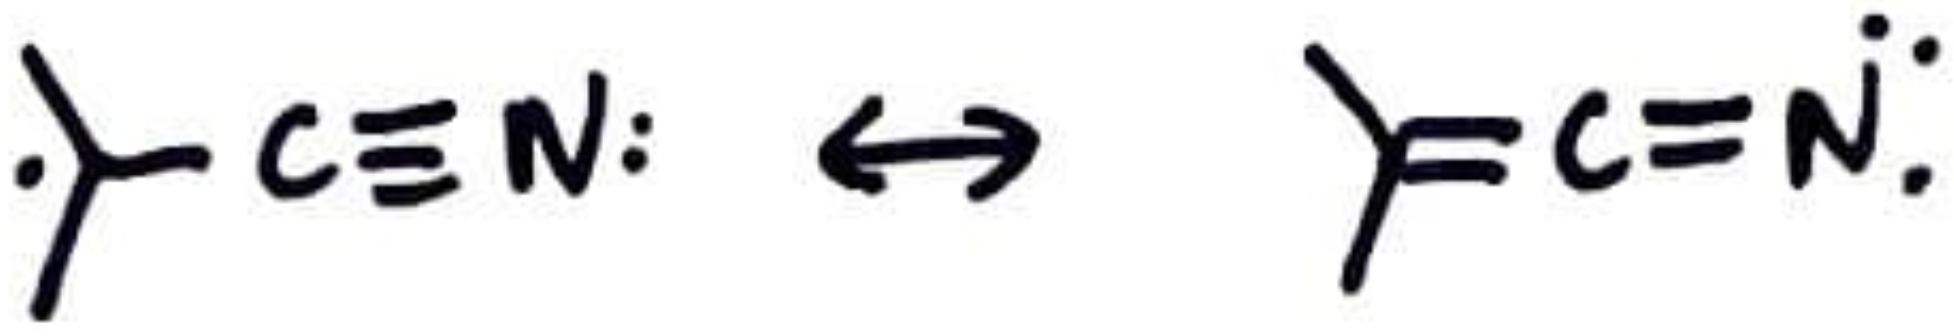
\includegraphics[width=0.8\linewidth]{radResc.png}
            \caption{Nitrile-adjacent radical.}
            \label{fig:radResc}
        \end{subfigure}
        \begin{subfigure}[b]{0.32\linewidth}
            \centering
            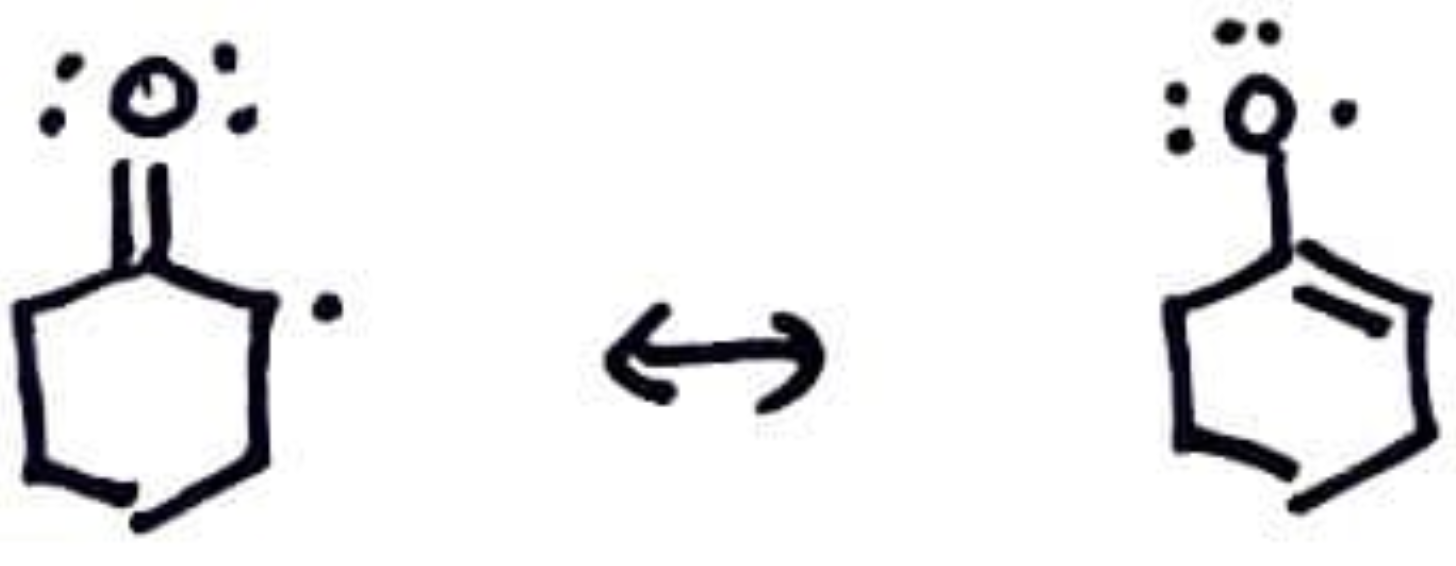
\includegraphics[width=0.7\linewidth]{radResd.png}
            \caption{Carbonyl-adjacent radical.}
            \label{fig:radResd}
        \end{subfigure}\\[2em]
        \begin{subfigure}[b]{\linewidth}
            \centering
            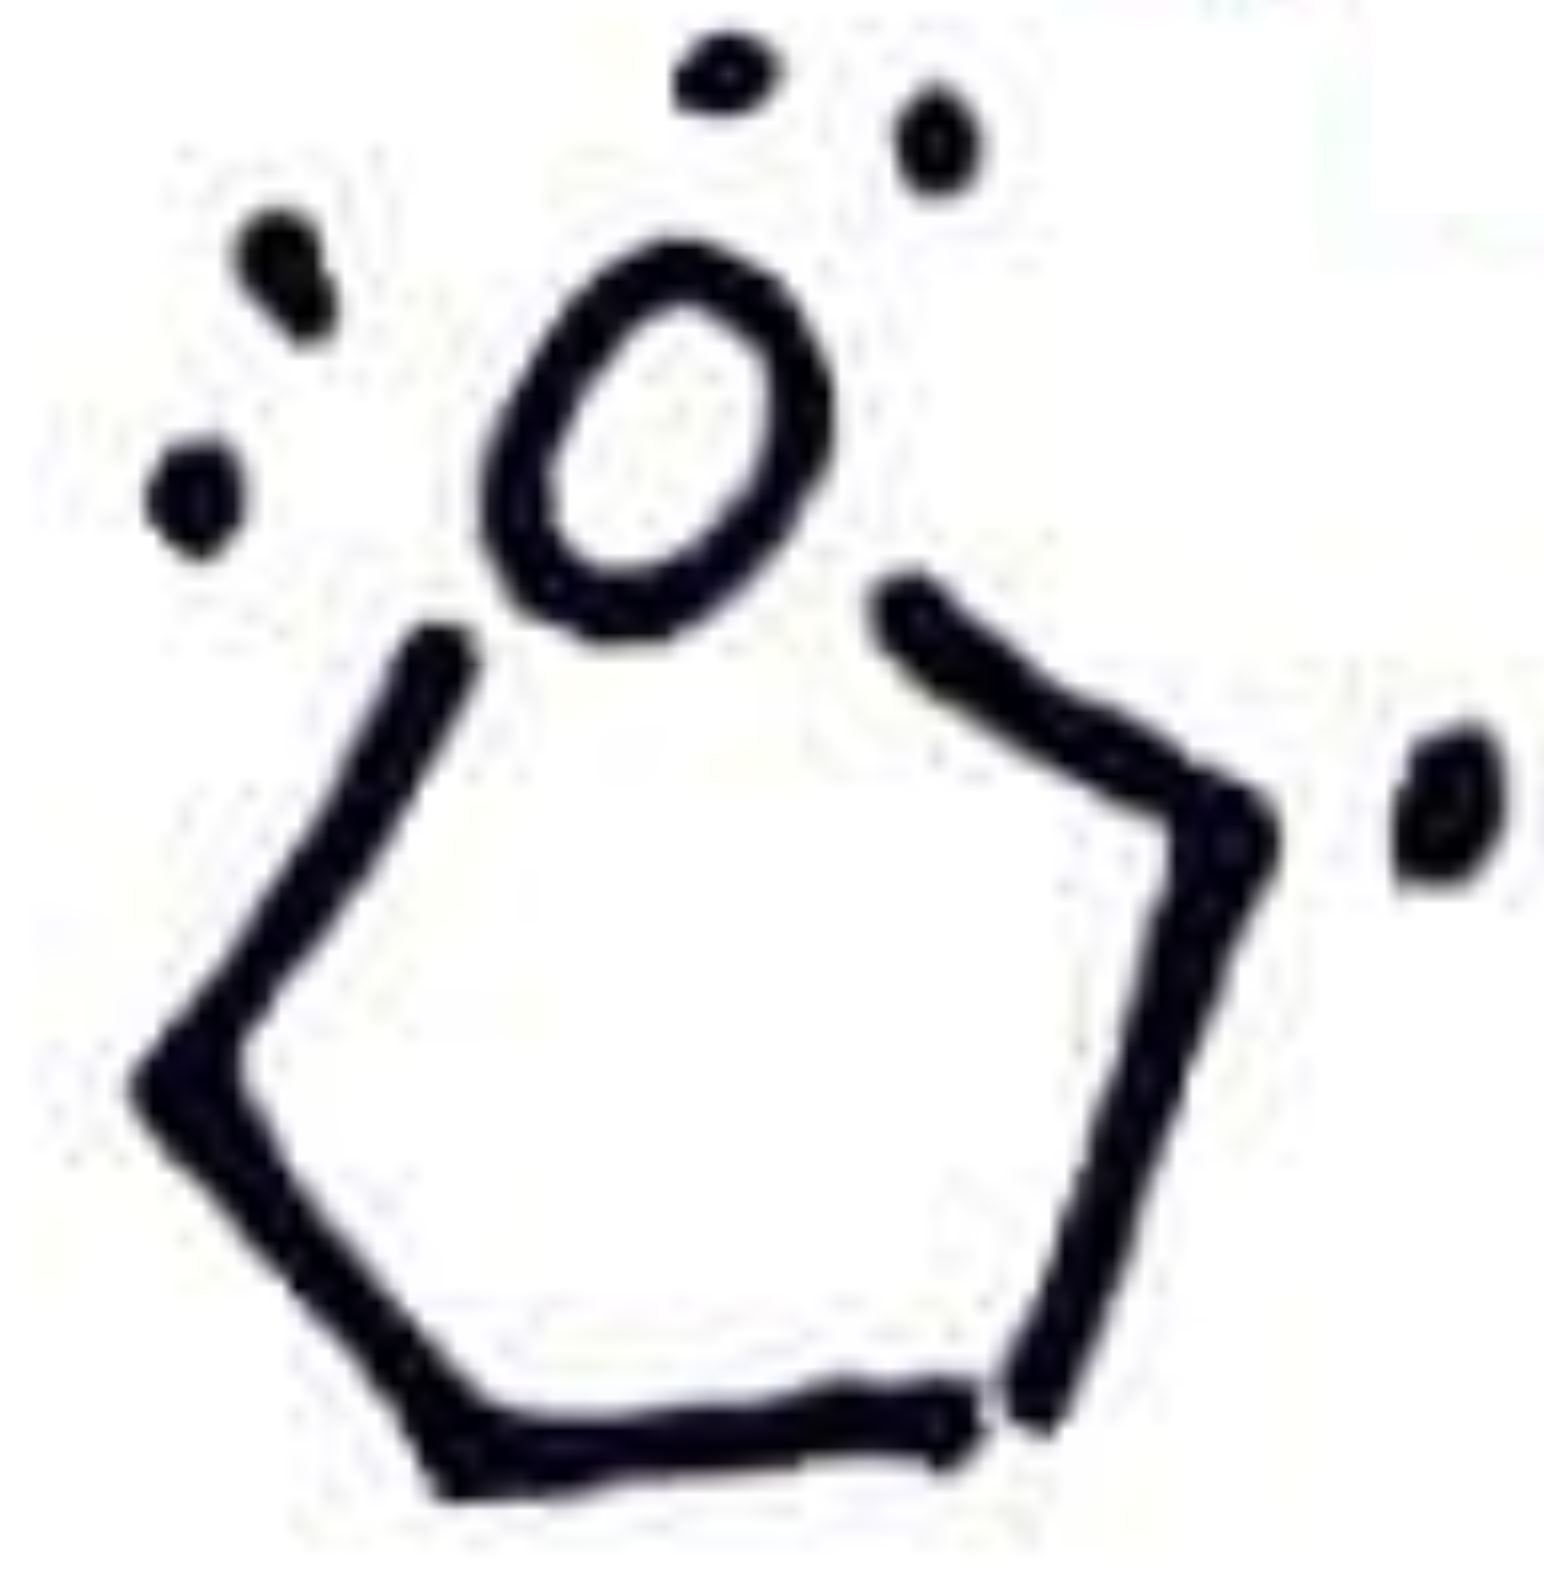
\includegraphics[width=0.055\linewidth]{radRese.png}
            \caption{Heteroatom-stabilized radical.}
            \label{fig:radRese}
        \end{subfigure}
        \caption{Resonance-stabilized radicals.}
        \label{fig:radRes}
    \end{figure}
    \begin{itemize}
        \item Allyl (Figure \ref{fig:radResa}) and benzyl (Figure \ref{fig:radResb}) radicals are also significantly stabilized, due to resonance.
        \begin{itemize}
            \item The allyl radical is \kcal{9} more stable than the propyl radical; \kcal{9} amounts to hundreds of times increased stability since each \kcal{1.4} is a 10-fold increase in stability.
        \end{itemize}
        \item Unlike many other electron-deficient species, electron-withdrawing groups actually stabilize radicals as well (Figures \ref{fig:radResc} \& \ref{fig:radResd})!
        \begin{itemize}
            \item This is because of resonance.
        \end{itemize}
        \item Lastly, radicals are also stabilized by lone pairs.
        \begin{itemize}
            \item This yields 2-centered, 3-electron bonding.
            \item Implication: Radicals $\alpha$ to an ether are stabilized. Here's why this is important.
            \begin{itemize}
                \item When you work in the lab (at MIT or elsewhere) and you buy an ether, the two most common ones to buy are tetrahydrofuran (THF) and diethyl ether (\ce{Et2O}).
                \item Once you open the container, you need to date it and then check it every six months for peroxides. These can form spontaneously in air, and then are dangerous because they're explosive!
            \end{itemize}
            \item An analogy to this is the stabilization of carbocations by resonance (see Figure \ref{fig:CCheteroatoma}).
        \end{itemize}
    \end{itemize}
    \item Unstable radicals.
    \begin{figure}[h!]
        \centering
        \footnotesize
        \begin{subfigure}[b]{0.2\linewidth}
            \centering
            \chemfig{*6(-=\charge{-30=\.}{}-=-=)}
            \caption{Phenyl radical.}
            \label{fig:radUnstablea}
        \end{subfigure}
        \begin{subfigure}[b]{0.2\linewidth}
            \centering
            \chemfig{=\charge{0=\.}{}}
            \caption{Vinyl radical.}
            \label{fig:radUnstableb}
        \end{subfigure}
        \begin{subfigure}[b]{0.2\linewidth}
            \centering
            \chemfig{~\charge{0=\.}{}}
            \caption{Acetylinic radical.}
            \label{fig:radUnstablec}
        \end{subfigure}
        \caption{Unstable radicals.}
        \label{fig:radUnstable}
    \end{figure}
    \begin{itemize}
        \item What these all have in common is that they must be generated by cleaving (in a homolytic sense) relatively strong \ce{C-H} bonds.
        \item In contrast, many of the radicals in Figure \ref{fig:radRes} derive from relative weaker \ce{C-H} bonds (in a homolytic sense).
    \end{itemize}
    \item Generation of radicals.
    \item Peroxides.
    \begin{figure}[h!]
        \centering
        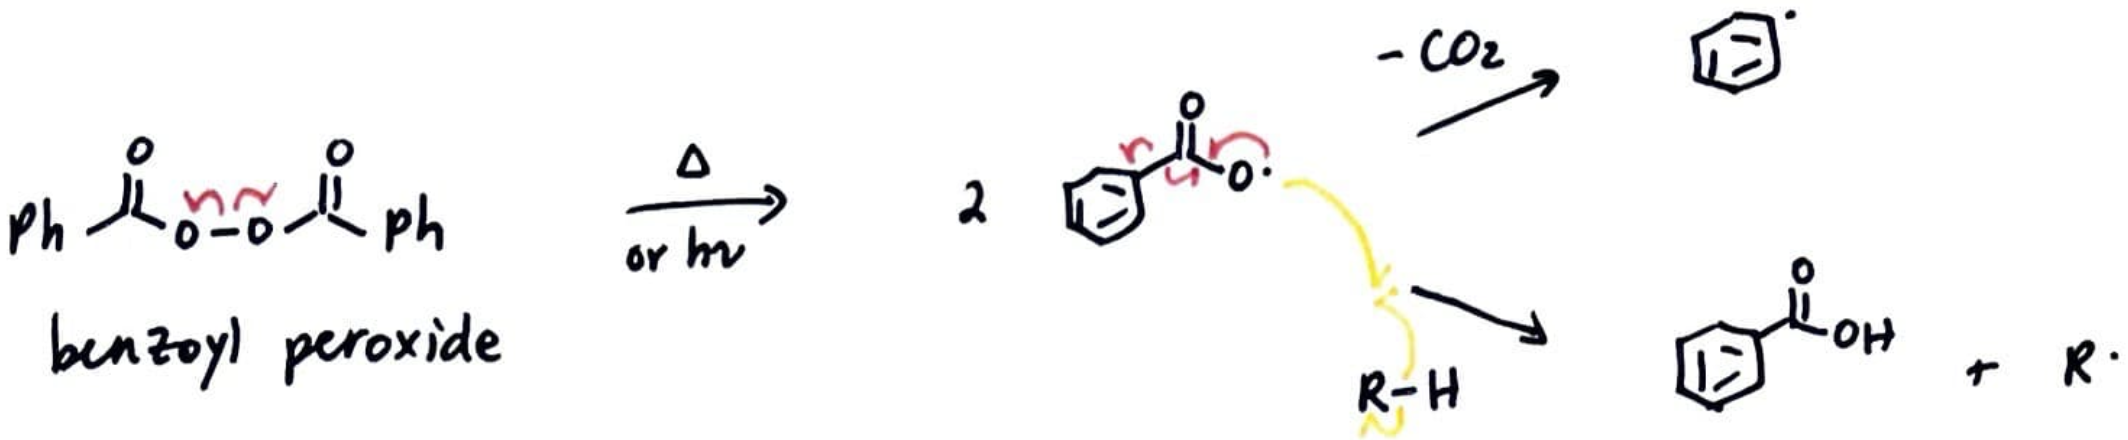
\includegraphics[width=0.8\linewidth]{radGenPeroxide.png}
        \caption{Generating radicals from peroxides.}
        \label{fig:radGenPeroxide}
    \end{figure}
    \begin{itemize}
        \item Many old acne medications contained benzoyl peroxide.
        \item The center \ce{O-O} bond is very weak: It's bond dissociation energy is only about \kcal{30}.
        \item Thus, under heat or light, the \ce{O-O} bond can break in two (we draw this using \emph{single-headed} curved arrows) to yield an intermediate.
        \item This intermediate will then either quickly do decarboxylation to form \ce{CO2} and a phenyl radical, or quickly grab hydrogen from a nearby \ce{R-H} to form benzoic acid and a \ce{R*} radical.
        \begin{itemize}
            \item Either process kills the bacteria in acne!
        \end{itemize}
    \end{itemize}
    \item Initiators.
    \begin{figure}[h!]
        \centering
        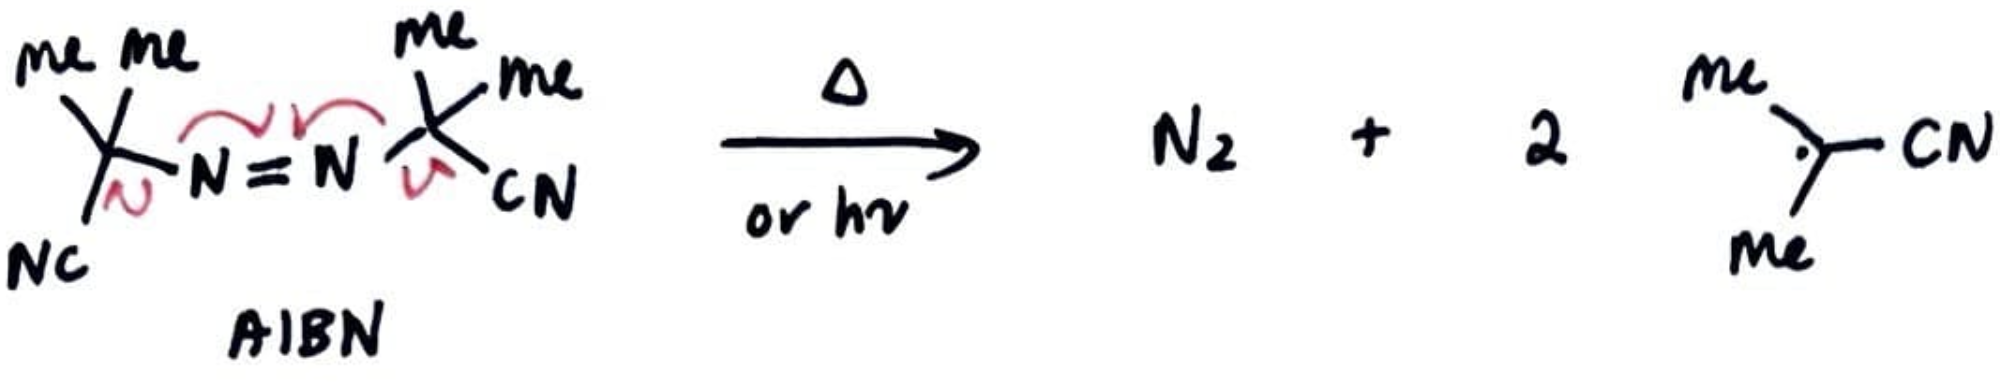
\includegraphics[width=0.55\linewidth]{radGenAIBN.png}
        \caption{Generating radicals from AIBN.}
        \label{fig:radGenAIBN}
    \end{figure}
    \begin{itemize}
        \item AIBN (azoisobutyronitrile) --- under light or heat --- forms nitrogen gas and two equivalents of a tertiary, resonance-stabilized radical (see Figure \ref{fig:radResd}).
    \end{itemize}
    \item We now move onto Topic B: Reactions of radicals.
    \item Radicals often participate in \textbf{radical chain reactions}.
    \begin{itemize}
        \item These are used in the synthesis of polymers, they're in our body, and we put things in our food to prevent them because food spoils via radical chain reactions.
    \end{itemize}
    \item We now discuss Topic B.1: Termination steps.
    \item \textbf{Termination} (step): A process that consumes radicals via mutual annihilation.
    \item We'll now cover Topic B.1.a{}: Radical-radical coupling.
    \begin{figure}[h!]
        \centering
        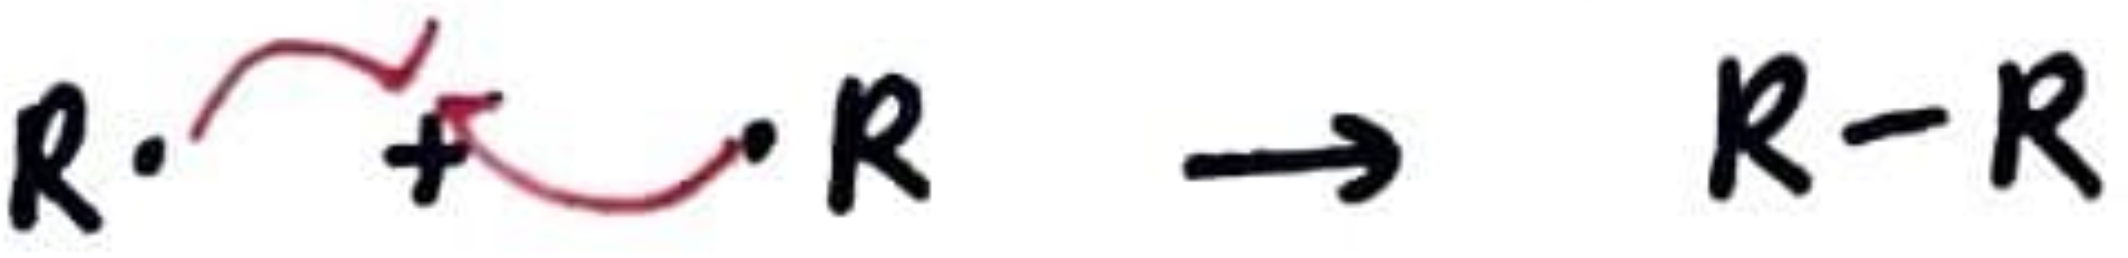
\includegraphics[width=0.24\linewidth]{radCoupling.png}
        \caption{Radical-radical coupling.}
        \label{fig:radCoupling}
    \end{figure}
    \item We now move onto Topic B.1.b{}: Disproportionation.
    \begin{figure}[H]
        \centering
        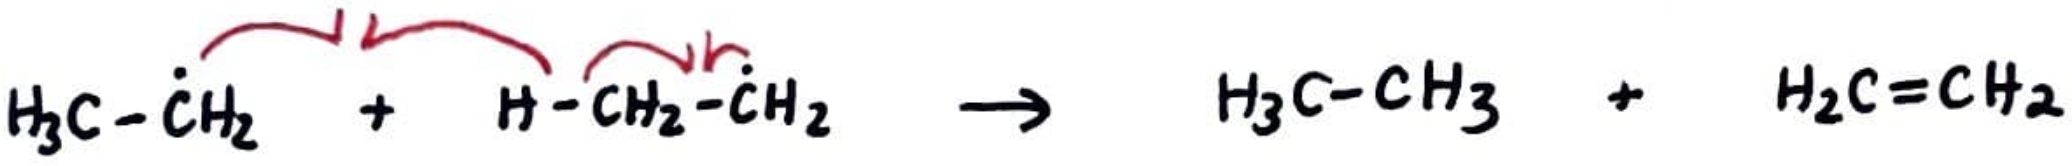
\includegraphics[width=0.59\linewidth]{radDisproport.png}
        \caption{Disproportionation.}
        \label{fig:radDisproport}
    \end{figure}
    \item We now move onto Topic B.2: Propagation steps.
    \item More specifically, we'll cover Topic B.2.a{}: Abstraction.
    \begin{figure}[h!]
        \centering
        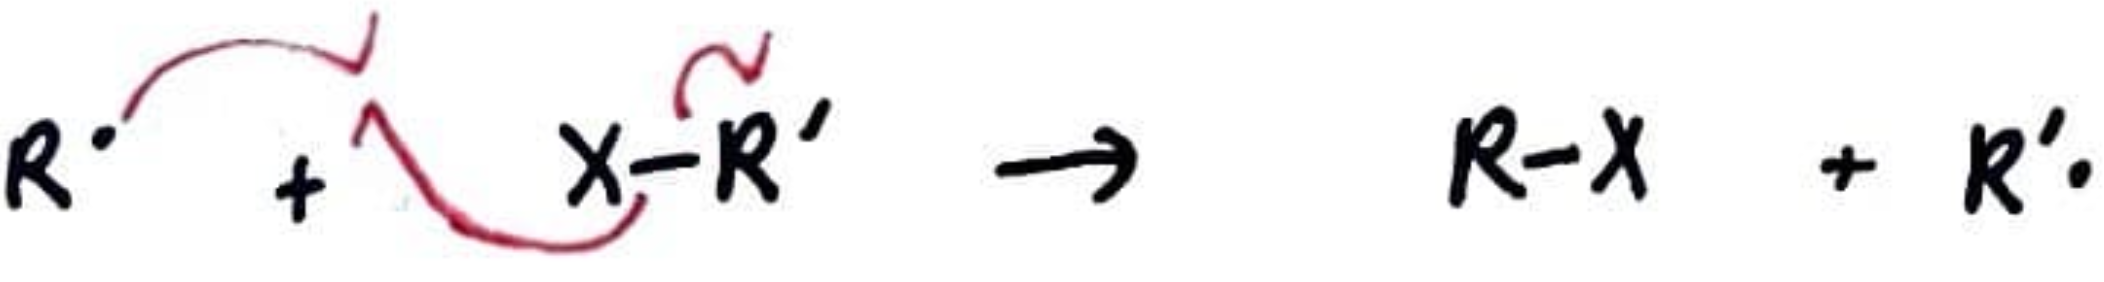
\includegraphics[width=0.37\linewidth]{radAbstract.png}
        \caption{Radical abstraction.}
        \label{fig:radAbstract}
    \end{figure}
    \begin{itemize}
        \item Also called S\textsubscript{H}2 (substitution, homolytic, bimolecular).
        \item This step continues the radical chain because we put one radical in and get one radical out.
    \end{itemize}
    \item We now move onto Topic B.2.b{}: Addition to double and triple bonds.
    \begin{figure}[h!]
        \centering
        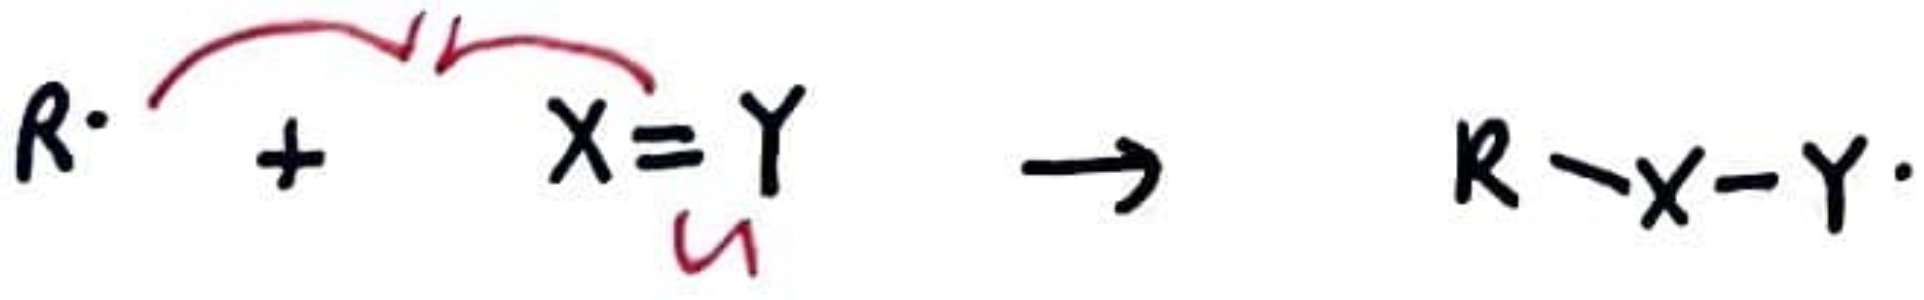
\includegraphics[width=0.33\linewidth]{radAddMult.png}
        \caption{Radical addition to multiple bonds.}
        \label{fig:radAddMult}
    \end{figure}
    \begin{itemize}
        \item We attack an \ce{X=Y} bond, attach to one atom (say \ce{X}), and form a \ce{Y}-centered radical.
    \end{itemize}
    \item We now move onto Topic B.2.c{}: Fragmentation.
    \begin{itemize}
        \item This is typified by the decarboxylation reaction in Figure \ref{fig:radGenPeroxide}.
    \end{itemize}
    \item We now move onto Topic B.2.d{}: Rearrangement.
    \begin{figure}[h!]
        \centering
        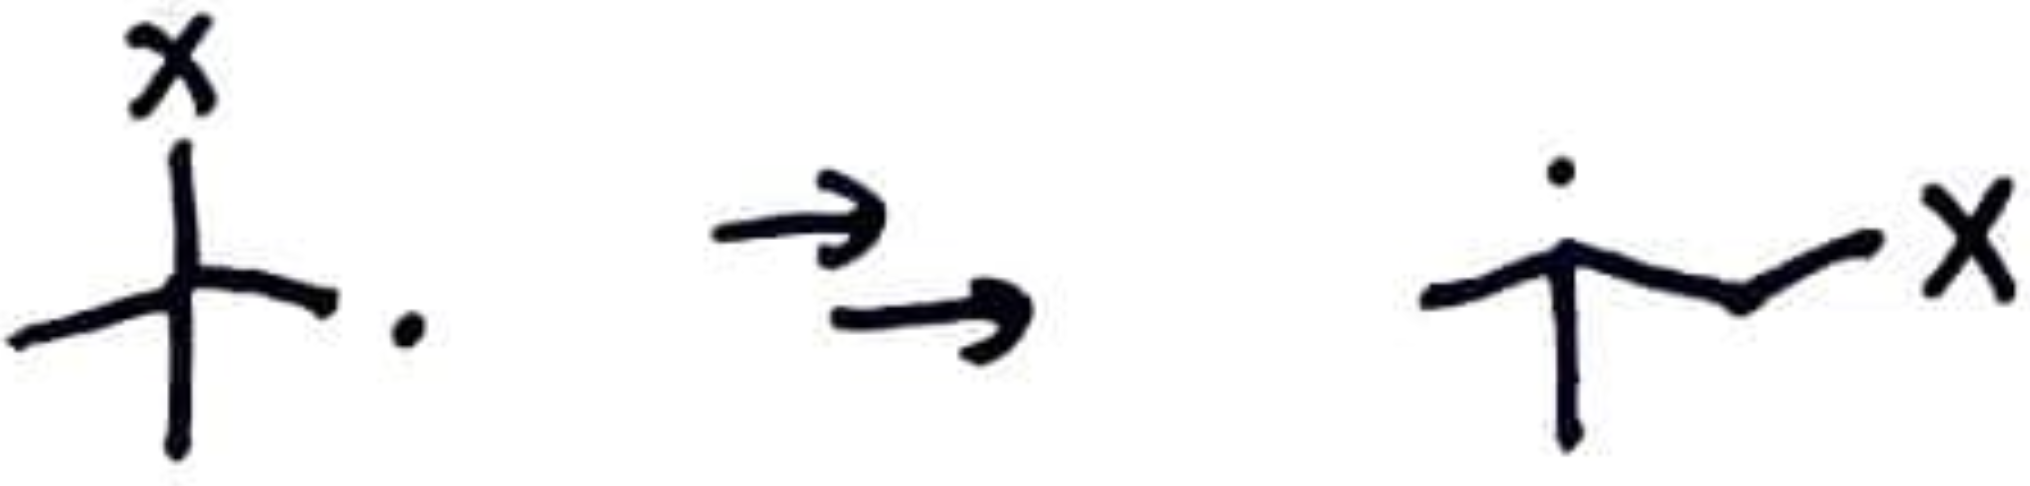
\includegraphics[width=0.24\linewidth]{radRearr.png}
        \caption{Radical rearrangement.}
        \label{fig:radRearr}
    \end{figure}
    \begin{itemize}
        \item This allows us to get to a more stable radical, e.g., $1^\circ\to 3^\circ$.
    \end{itemize}
    \item Radical fragmentation and rearrangement, in particular, are usually \emph{very fast} processes.
    \item We now move onto Topic B.3: Radical chain reactions.
    \begin{itemize}
        \item These have three steps: Initiation, propagation, and termination.
    \end{itemize}
    \item Example radical chain reaction: Radical reduction.
    \begin{figure}[h!]
        \centering
        \footnotesize
        \schemestart
            \chemfig{R-Br}
            \+
            \chemfig{Bu_3Sn-H}
            \arrow{->[cat. AIBN][\SI{80}{\celsius}]}[,1.5]
            \chemfig{R-H}
            \+
            \chemfig{Bu_3Sn-Br}
        \schemestop
        \caption{Radical reduction of alkyl halides.}
        \label{fig:radRXreduce}
    \end{figure}
    \begin{itemize}
        \item Combine \ce{R-Br} and \ce{Bu3Sn-H} with a catalytic amount of AIBN at \SI{80}{\celsius}.
        \begin{itemize}
            \item Every butyl group is \emph{n}-butyl, but Prof. Buchwald won't write out all the n's.
        \end{itemize}
        \item This reduces the alkyl halide to an alkyl group!
        \item Energetic analysis.
        \begin{itemize}
            \item Bond dissociation energies (BDEs).
            \begin{itemize}
                \item The \ce{R-Br} bond has a BDE of about \kcal{70}.
                \item The \ce{Bu3Sn-H} bond has a BDE of about \kcal{74}.
                \item The \ce{R-H} bond in the product has a BDE of about \kcal{95}.
                \item The \ce{Bu3Sn-Br} bond in the product has a BDE of about \kcal{85}.
            \end{itemize}
            \pagebreak
            \item Thus, via Hess's law, this reaction is thermodynamically favorable overall by \kcal{36}!
        \end{itemize}
        \item However, if we just mix the reactants, nothing happens because of the \emph{kinetic} barrier.
        \begin{itemize}
            \item This is why we add a catalytic amount of AIBN.
            \item Note that we do mean "catalytic amount" and not "catalyst": AIBN is consumed in the reaction and not regenerated (per Figure \ref{fig:radGenAIBN}), so it is not technically a catlyst.
        \end{itemize}
    \end{itemize}
    \item Let's now discuss the mechanism of the above reaction.
    \begin{figure}[h!]
        \centering
        \begin{subfigure}[b]{\linewidth}
            \centering
            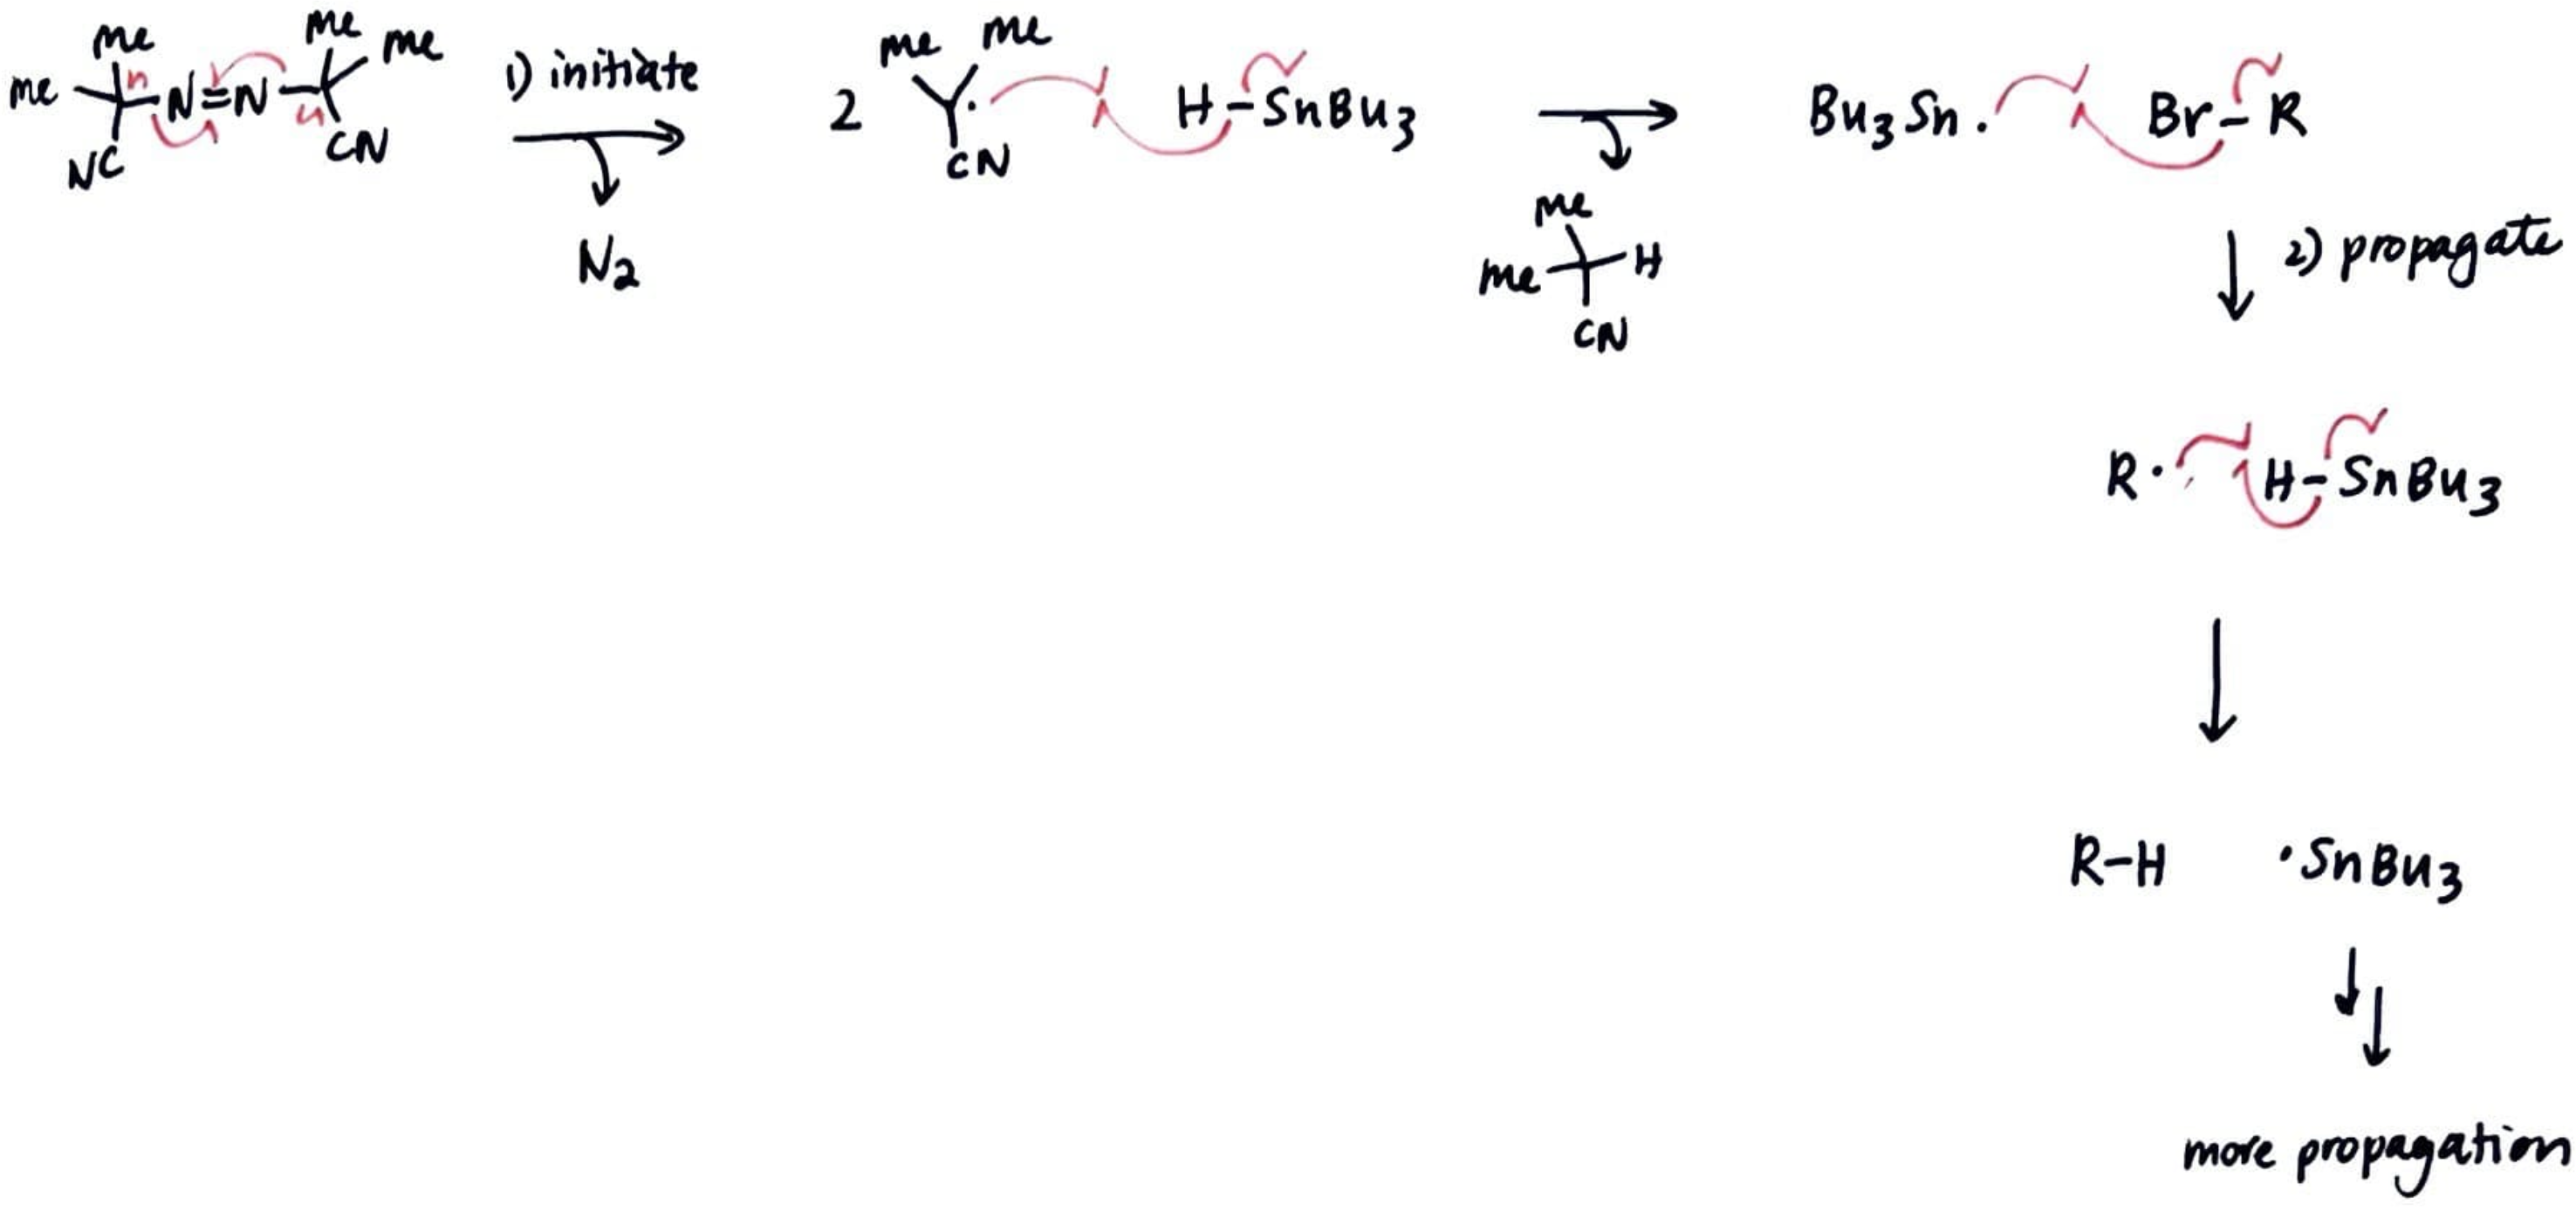
\includegraphics[width=0.93\linewidth]{radRXreduceMecha.png}
            \caption{Initiation and propagation steps.}
            \label{fig:radRXreduceMecha}
        \end{subfigure}\\[2em]
        \begin{subfigure}[b]{\linewidth}
            \centering
            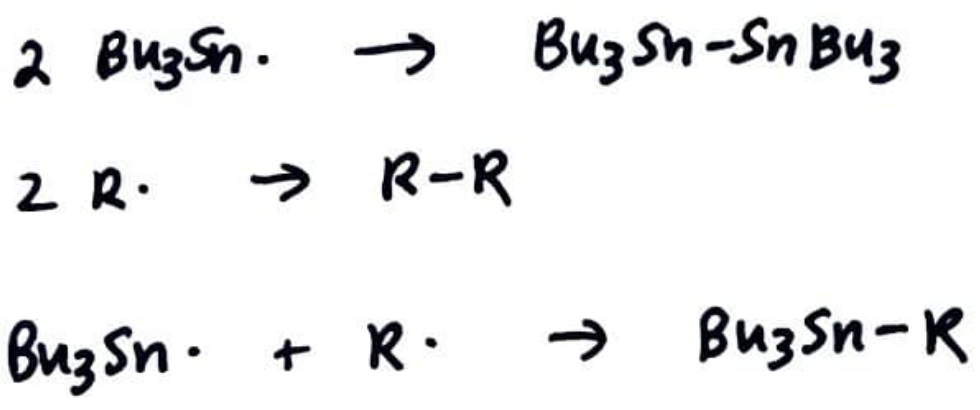
\includegraphics[width=0.3\linewidth]{radRXreduceMechb.png}
            \caption{Possible termination steps.}
            \label{fig:radRXreduceMechb}
        \end{subfigure}
        \caption{Radical reduction mechanism.}
        \label{fig:radRXreduceMech}
    \end{figure}
    \begin{itemize}
        \item First, AIBN will undergo its initiation reaction (see Figure \ref{fig:radGenAIBN}).
        \item The radicals generated by this initiation step go after the weak \ce{Bu3Sn-H} bond, generated a tributylstannyl (\ce{Bu3Sn*}) radical.
        \item These tin radicals then like to go after halogens because \ce{Sn-X} bonds are \emph{strong}.
        \begin{itemize}
            \item Thus, this step is favorable by about \kcal{15}!
        \end{itemize}
        \item Then the \ce{R*} radical can go after the next molecule of \ce{Bu3Sn-H} to regenerate \ce{Bu3Sn*} (to react further) as well as a molecule of the \ce{R-H} product.
        \begin{itemize}
            \item This step is favorable by about \kcal{21}.
        \end{itemize}
        \item Adding up the propagation steps both thermodynamically and molecule-by-molecule gives our net reaction and $\Delta H=-\kcal{36}$.
        \item Termination steps.
        \begin{itemize}
            \item Radical-radical coupling (see Figure \ref{fig:radCoupling}) of \ce{Bu3Sn*} radicals, \ce{R*} radicals, and \ce{Bu3Sn* + R*}.
            \item For a radical chain process to be efficient, we want propagation to occur around a hundred times before termination occurs.
        \end{itemize}
    \end{itemize}
\end{itemize}




\end{document}